\section{Arquitectura del sistema}
\label{sec:arquitectura-e4}

Esta sección documenta la arquitectura resultante tras la Entrega 4 en los tres niveles del
modelo C4~\cite{brown2018c4model}, y resume las decisiones registradas como \emph{Architectural
Decision Records} (ADR) que la sustentan.

\subsection{Vista de contexto (C4 Nivel 1)}

La Figura~\ref{fig:c4-nivel1} sitúa el sistema como una sola caja frente a sus tres tipos de
usuario. No hay sistemas externos reales que integrar en este nivel: lo que podría parecer una
integración externa —notificaciones multicanal, telemetría de equipos del abonado— está simulado
dentro del propio sistema y documentado como tal en cada ADR correspondiente (ver
\texttt{docs/diagrams/c4-nivel1-contexto.md} para el detalle de por qué).

\begin{figure}[H]
\centering
\includegraphics[width=0.85\textwidth]{../diagrams/c4-nivel1-contexto.png}
\caption{C4 Nivel 1 — contexto del sistema.}
\label{fig:c4-nivel1}
\end{figure}

\subsection{Vista de contenedores (C4 Nivel 2)}

El diagrama de contenedores de la Entrega 3 (\texttt{docs/diagrams/c4-nivel2-contenedores.md})
se actualiza en esta entrega con las piezas nuevas: las dos
aplicaciones cliente (\texttt{apps/web}, \texttt{apps/mobile}) ya no hablan directamente con cada
microservicio por su puerto, sino que pasan por un único \texttt{api-gateway} (Spring Cloud
Gateway) que enruta por prefijo de \emph{path} sin reescribir el cuerpo de la petición. Se agrega
\texttt{telemetry-service} (PE-U1, Sección~\ref{sec:pe-u1-correl}) como séptimo microservicio, y
el stack de observabilidad (OpenTelemetry Collector, Tempo, Prometheus, Grafana, cAdvisor) como
un grupo de contenedores transversal. La Figura~\ref{fig:c4-nivel2} muestra el diagrama completo.

\begin{figure}[H]
\centering
\includegraphics[width=\textwidth,height=0.92\textheight,keepaspectratio]{../diagrams/c4-nivel2-contenedores.png}
\caption{C4 Nivel 2 — contenedores del sistema, Entrega 4.}
\label{fig:c4-nivel2}
\end{figure}

\begin{table}[H]
\centering
\small
\caption{Contenedores del sistema tras la Entrega 4.}
\label{tab:contenedores-e4}
\begin{tabular}{@{}p{3.1cm}p{2.6cm}p{7.8cm}@{}}
\toprule
\textbf{Contenedor} & \textbf{Tecnología} & \textbf{Responsabilidad} \\
\midrule
\texttt{apps/web} & React 18 + TypeScript & SPA de consola para clientes/técnicos/administradores \\
\texttt{apps/mobile} & Kotlin + Jetpack Compose & Cliente de campo para técnicos (APK) \\
\texttt{api-gateway} & Spring Cloud Gateway & Único punto de entrada, enrutamiento por prefijo \\
\texttt{auth-service} & Java 21 + Spring Boot & JWT, RBAC, refresh tokens \\
\texttt{ticket-service} & Java 21 + Spring Boot & CRUD de tickets, arquitectura hexagonal (Sección~\ref{sec:hexagonal-e4}) \\
\texttt{ai-service} & Python + FastAPI & Clasificación asíncrona por reglas \\
\texttt{notification-service} & Node.js + Express & Notificaciones multicanal simuladas \\
\texttt{report-service} & Java 21 + Spring Boot & Modelo de lectura CQRS, reportes \\
\texttt{telemetry-service} & Java 21, sockets TCP + gRPC & Canal PE-U1: equipos del abonado + latidos de nodo, reloj de Lamport (Sección~\ref{sec:pe-u1-correl}) \\
CockroachDB & Cluster 3 nodos & Persistencia distribuida (auth\_db/ticket\_db/report\_db) \\
Kafka + MongoDB & --- & Saga por coreografía, clasificaciones y notificaciones \\
OTel Collector, Tempo, Prometheus, Grafana, cAdvisor & --- & Observabilidad (Sección~\ref{sec:observabilidad}) \\
\bottomrule
\end{tabular}
\end{table}

\subsection{Vista de componentes (C4 Nivel 3)}
\label{sec:c4-nivel3}

El único servicio con arquitectura hexagonal completa es \texttt{ticket-service}
(Sección~\ref{sec:hexagonal-e4}), así que es el que se documenta en este nivel del modelo:
zoom a sus componentes reales, no a una aproximación. La Figura~\ref{fig:c4-nivel3} —fuente
versionada en \texttt{docs/diagrams/c4-nivel3-componentes.md}— nombra cada caja igual que el
árbol de \texttt{services/svc-principal/src/main/java/.../ticketservice/}: los seis patrones GoF
de la Sección~\ref{sec:gof-e4} son visibles aquí, no solo enumerados en prosa.

La imagen fuente (\texttt{docs/diagrams/c4-nivel3-componentes.png}) es extremadamente alargada
(1109×4348~px, relación de aspecto 1:4) porque Mermaid apila las 27 cajas en una sola columna
vertical. Encajada como una sola figura en una página vertical (con la altura acotada al 85\,\% de la
altura de página), el ancho resultante quedaba en apenas ~5~cm, con el texto de cada caja en torno a 1,4~pt
impreso —ilegible, aunque la imagen en sí no perdiera contenido— (hallazgo de una revisión
externa). Se divide aquí en cuatro franjas horizontales iguales, de arriba a abajo, sin recortar
ni omitir ninguna caja, dispuestas en una cuadrícula de $2\times2$ para que cada franja quede
acotada por el ancho de página (el lado que faltaba aprovechar) en vez de por la altura:

\begin{figure}[H]
\centering
\begin{minipage}{0.48\textwidth}
  \centering
  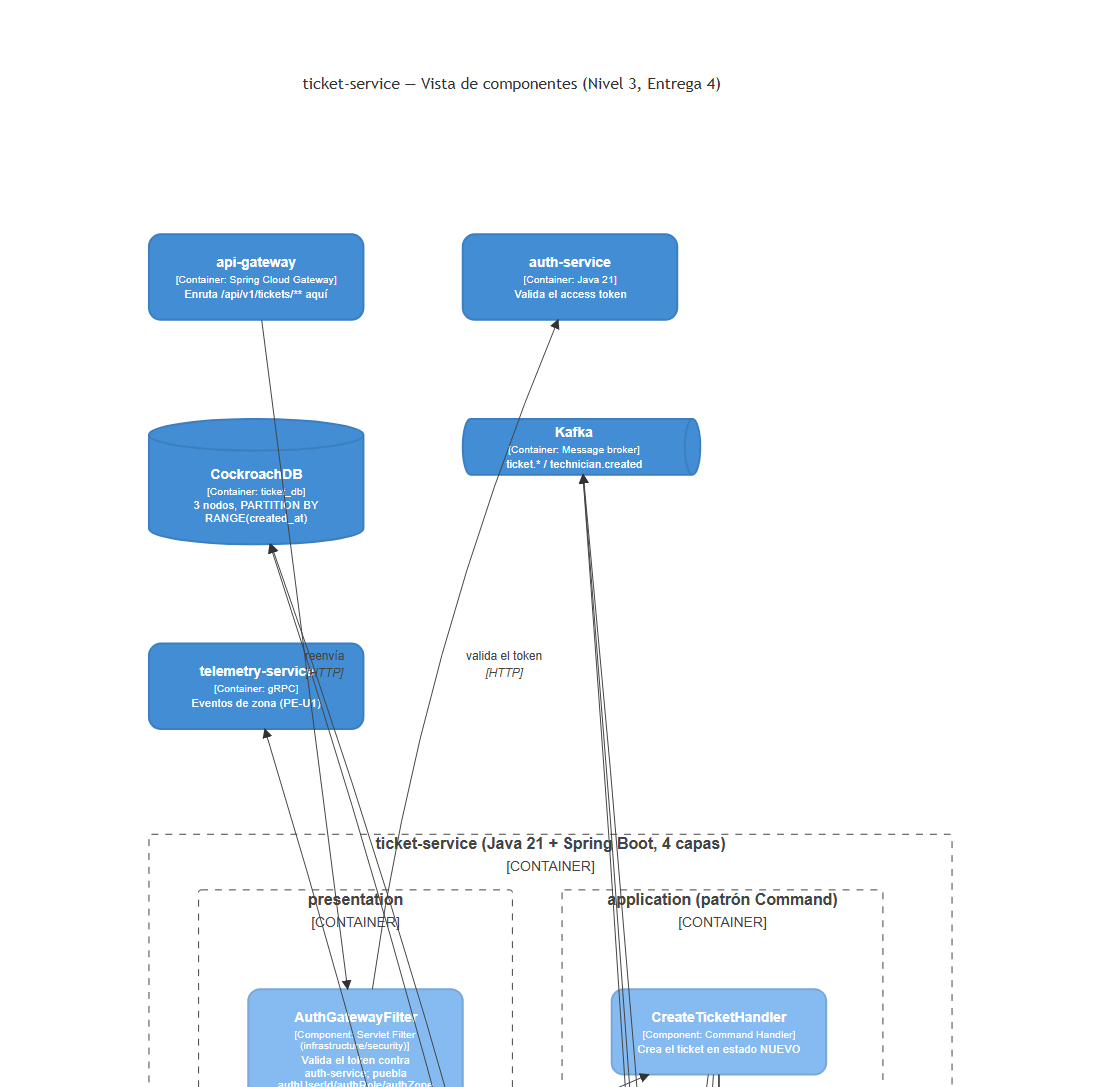
\includegraphics[width=\linewidth]{../diagrams/c4-nivel3-componentes-parte1.png}
  \\ \footnotesize (a)
\end{minipage}
\hfill
\begin{minipage}{0.48\textwidth}
  \centering
  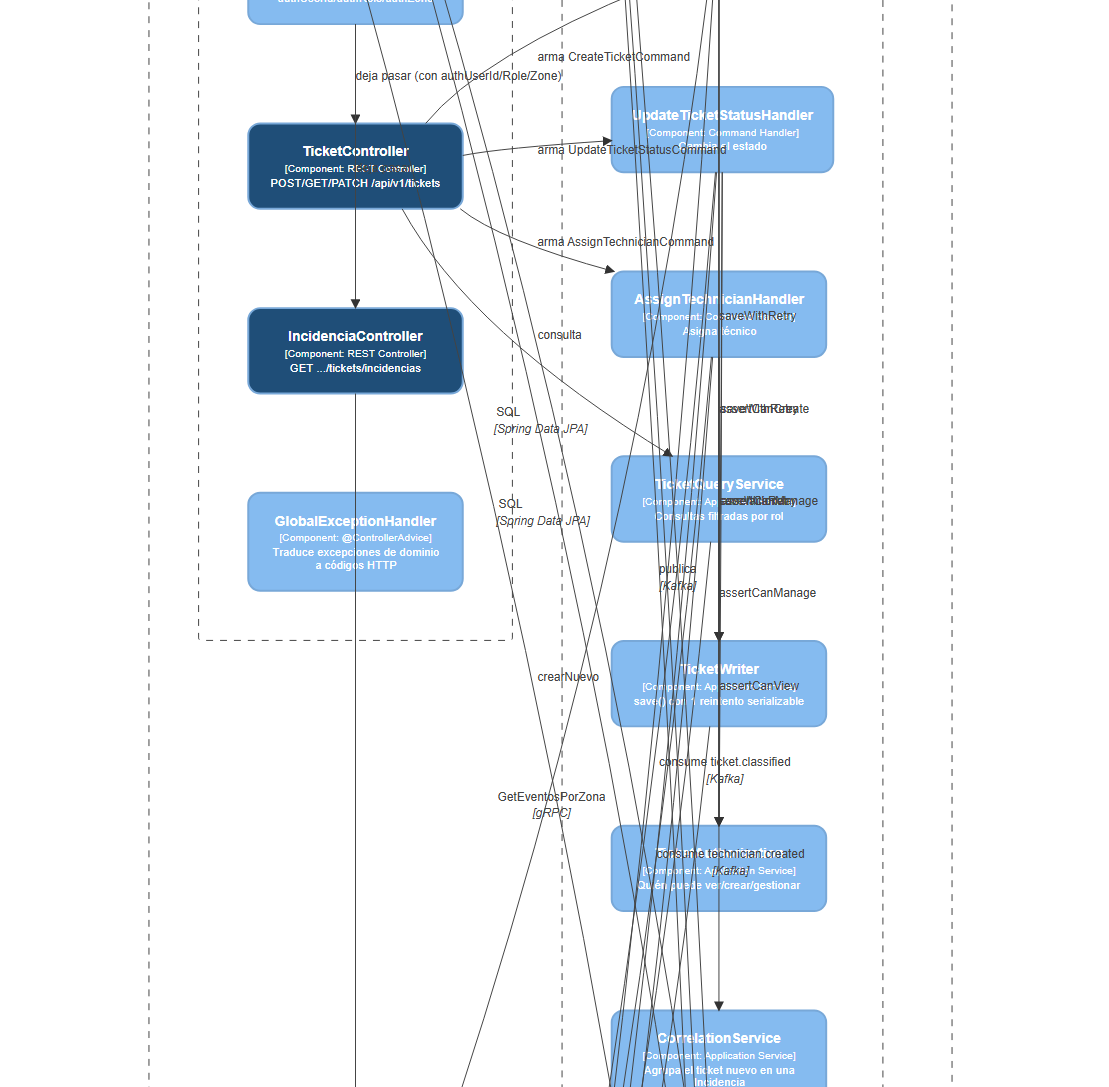
\includegraphics[width=\linewidth]{../diagrams/c4-nivel3-componentes-parte2.png}
  \\ \footnotesize (b)
\end{minipage}

\vspace{4pt}
\begin{minipage}{0.48\textwidth}
  \centering
  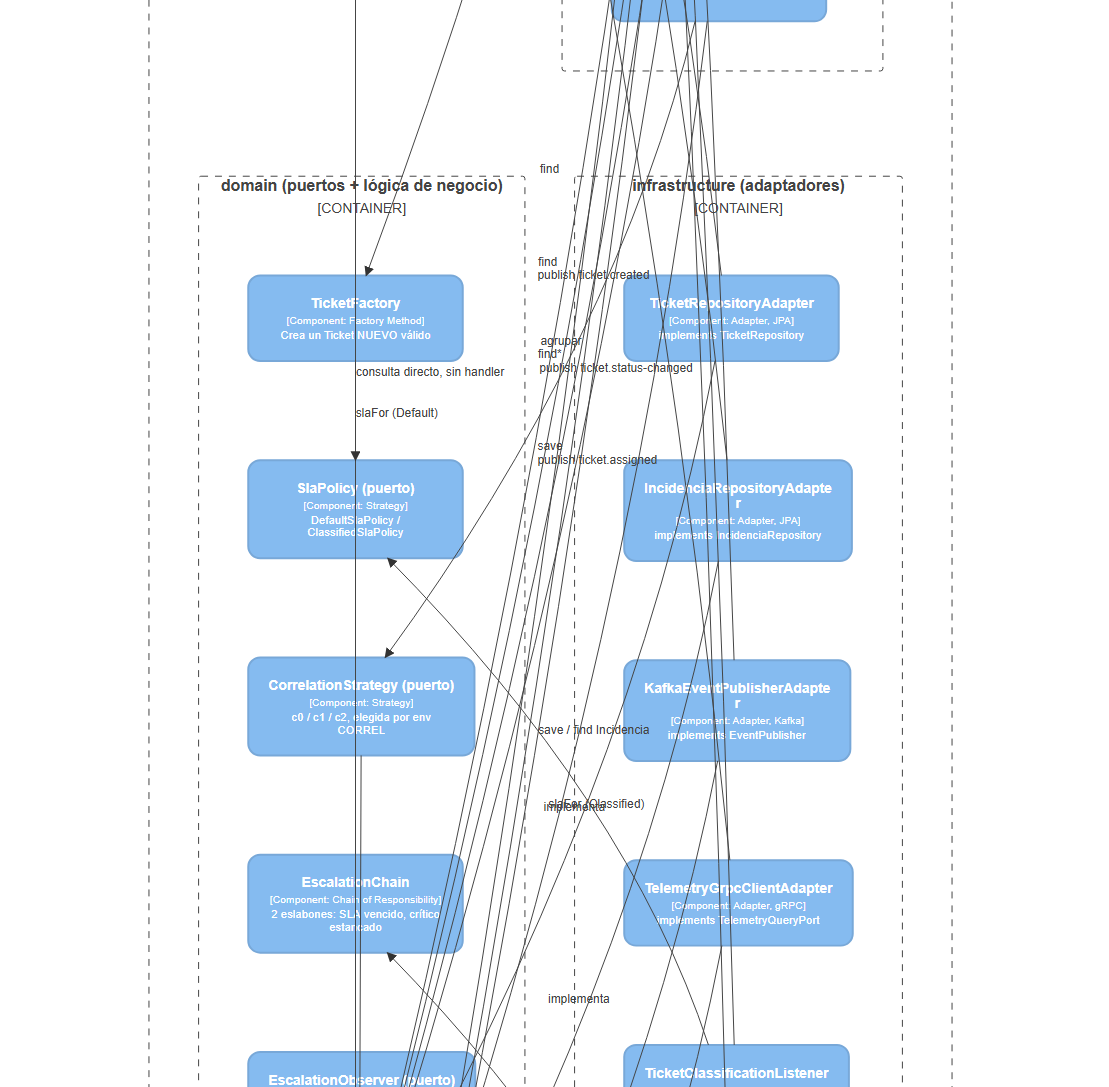
\includegraphics[width=\linewidth]{../diagrams/c4-nivel3-componentes-parte3.png}
  \\ \footnotesize (c)
\end{minipage}
\hfill
\begin{minipage}{0.48\textwidth}
  \centering
  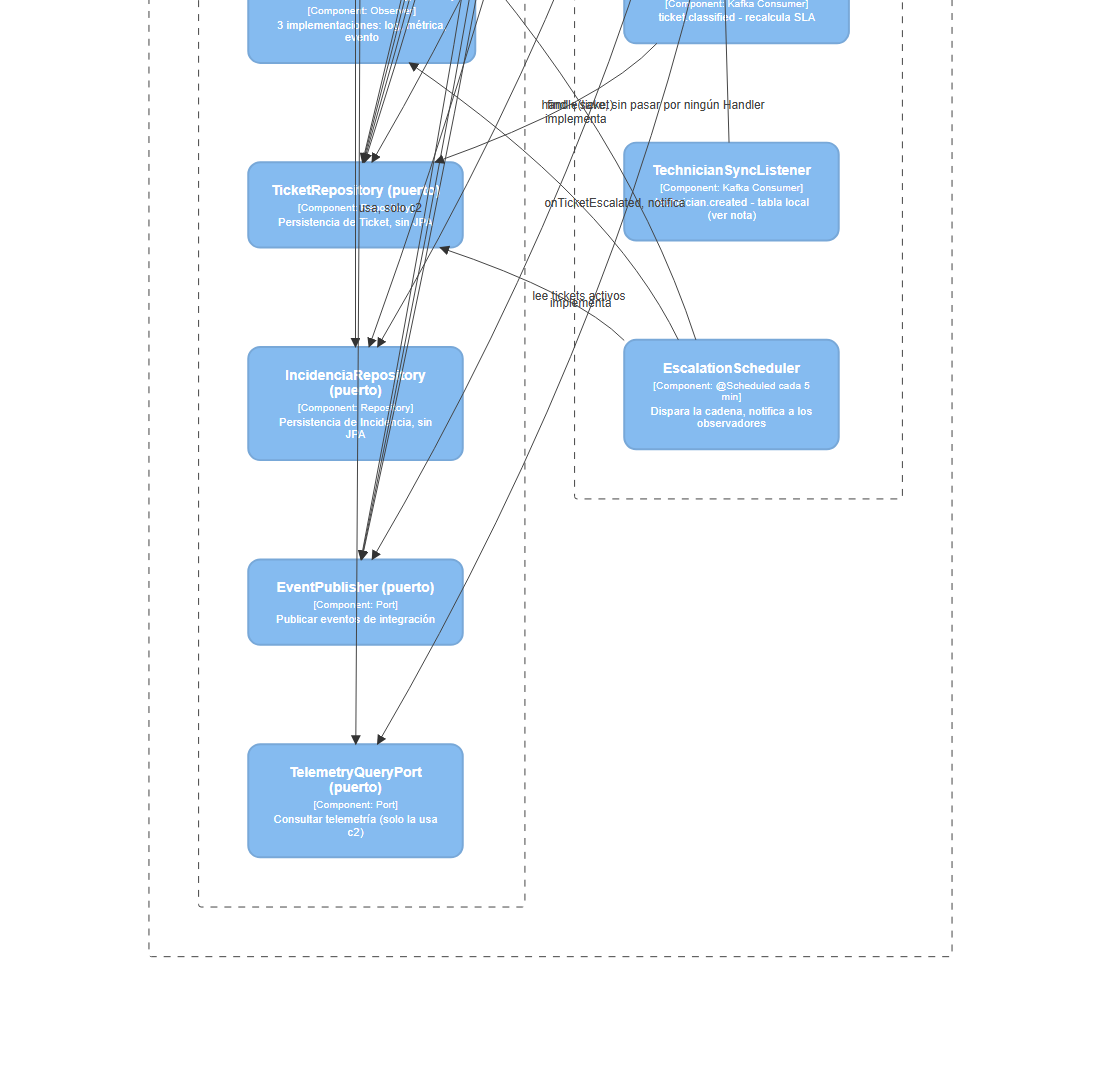
\includegraphics[width=\linewidth]{../diagrams/c4-nivel3-componentes-parte4.png}
  \\ \footnotesize (d)
\end{minipage}
\caption{C4 Nivel 3 — componentes de \texttt{ticket-service}, Entrega 4. Mismo diagrama que
\texttt{c4-nivel3-componentes.png}, dividido en cuatro franjas horizontales (a)--(d), de arriba
a abajo, para que el texto de cada caja sea legible en la página.}
\label{fig:c4-nivel3}
\end{figure}

Dos rutas del diagrama rompen deliberadamente la capa de aplicación, documentado en vez de
ocultado: \texttt{IncidenciaController} consulta \texttt{IncidenciaRepository} directo (es una
lectura simple, sin caso de uso que orquestar), y \texttt{TicketClassificationListener} opera
sobre \texttt{TicketRepository} sin pasar por ningún \texttt{*CommandHandler} (el caso de uso
real es aplicar una clasificación asíncrona llegada por Kafka, no una acción HTTP con
autorización de rol). \texttt{TechnicianSyncListener} tampoco tiene puerto de dominio: escribe
directo en una tabla de sincronización local que no representa un concepto propio de
\texttt{ticket-service} --es una réplica de solo lectura de datos de \texttt{auth-service},
necesaria para que \texttt{AssignTechnicianHandler} no viole la clave foránea
\texttt{tickets\_technician\_id\_fkey}.

Construir este diagrama contra el árbol real, y no contra la descripción en prosa que ya existía,
encontró además una discrepancia en la Tabla~\ref{tab:capas-e4}: decía que \texttt{domain} tiene
``cero anotaciones Spring/JPA''. Verificado con \texttt{grep} sobre el paquete: era falso para la
parte de Spring --12 líneas \texttt{import org.springframework.*} en 9 clases
(\texttt{@Component}, \texttt{@Value}, \texttt{@Order}, todas para que Spring descubra e inyecte
cada implementación de un puerto)-- aunque cierto para JPA, que no aparece en ningún archivo de
\texttt{domain}. Se movieron esas doce líneas a
\texttt{infrastructure/config/DomainBeansConfig.java} (Sección~\ref{sec:hexagonal-e4}), y se
agregó una prueba ArchUnit (\texttt{architecture/DomainArchitectureTest.java}) que falla la
construcción si \texttt{domain} vuelve a depender de Spring o de JPA -- ya no depende de que
alguien lo note leyendo el código a mano.

\subsection{Arquitectura hexagonal extendida}
\label{sec:hexagonal-e4}

El Módulo A de esta entrega exigió refactorizar el microservicio principal en cuatro capas con
una regla de dependencia estricta: las capas externas dependen de las internas, nunca al revés.
Antes del refactor, una única clase \texttt{TicketService} mezclaba acceso a datos vía
\texttt{JpaRepository} inyectado directamente, la lógica de creación de tickets en línea, dos
copias distintas del cálculo de SLA, y los tres casos de uso mutables como métodos sin forma
uniforme de interceptarlos.

\begin{table}[H]
\centering
\small
\caption{Las cuatro capas de \texttt{ticket-service} tras el refactor.}
\label{tab:capas-e4}
\begin{tabular}{@{}p{2.6cm}p{5.8cm}p{5.1cm}@{}}
\toprule
\textbf{Capa} & \textbf{Contenido} & \textbf{Regla} \\
\midrule
\texttt{presentation} & \texttt{TicketController}, DTOs & Traduce HTTP $\leftrightarrow$ comandos; sin lógica de negocio \\
\texttt{application} & \texttt{*CommandHandler} & Orquesta el caso de uso; no conoce HTTP ni JPA \\
\texttt{domain} & \texttt{Ticket}, puertos, políticas & Cero anotaciones Spring/JPA, verificado
  con una prueba ArchUnit que rompe la construcción si deja de serlo (ver
  Sección~\ref{sec:c4-nivel3}); se prueba con JUnit puro \\
\texttt{infrastructure} & Adaptadores, filtros, métricas, \emph{scheduler} & Implementa los puertos del dominio contra CockroachDB, Kafka y HTTP \\
\bottomrule
\end{tabular}
\end{table}

La regla de dependencia estricta ("las capas externas dependen de las internas, nunca al
revés") tampoco se verificaba de forma automática más allá de la ausencia de anotaciones de
Spring en \texttt{domain}: una revisión externa encontró que \texttt{TicketWriter}
(\texttt{application/}) importaba directamente \texttt{CrdbMetrics}
(\texttt{infrastructure/metrics/}) para incrementar un contador de reintentos, violando la
regla que esta misma tabla declara, sin que \texttt{DomainArchitectureTest} lo detectara. Se
corrigió con inversión de dependencias: \texttt{application/TransactionRetryMetrics.java} es
ahora el puerto que \texttt{TicketWriter} conoce, y \texttt{CrdbMetrics} lo implementa; Spring
sigue inyectando la implementación real por tipo. \texttt{DomainArchitectureTest} se amplió con
una regla de \texttt{Architectures.layeredArchitecture()} que verifica la dirección real de las
cuatro capas (\texttt{domain} $\leftarrow$ \texttt{application} $\leftarrow$
\texttt{infrastructure}/\texttt{presentation}), con una única excepción declarada:
\texttt{infrastructure} puede depender de \texttt{presentation} porque
\texttt{AuthGatewayFilter} reutiliza el sobre de respuesta \texttt{ApiResponse} para las
respuestas 401/403 que rechaza antes de que la petición llegue a un controlador.

Una revisión externa del repositorio observó, con razón, que este refactor completo solo se
había aplicado a \texttt{ticket-service}: los otros seis microservicios seguían con la
organización heredada de la Entrega 2 o de su propio diseño original (\texttt{telemetry-service}
es nuevo de esta entrega, sin arrastrar nada de E2). Se extendió el mismo patrón a
\texttt{auth-service} y \texttt{report-service} --los de menor superficie de los seis
restantes-- dejando explícitamente fuera de alcance \texttt{ai-service},
\texttt{notification-service}, \texttt{api-gateway} y \texttt{telemetry-service} por el tiempo
disponible antes del cierre; se documenta el alcance real en vez de sugerir un refactor completo
que no ocurrió.

\begin{table}[H]
\centering
\small
\caption{Alcance real del refactor a cuatro capas, y la violación concreta que corrigió en cada
caso.}
\label{tab:hexagonal-alcance}
\begin{tabular}{@{}p{2.9cm}p{4.6cm}p{6.0cm}@{}}
\toprule
\textbf{Servicio} & \textbf{Estado} & \textbf{Violación real corregida} \\
\midrule
\texttt{ticket-service} & 4 capas + 6 patrones GoF & \texttt{TicketService} mezclaba JPA, SLA y
  los tres casos de uso en una sola clase (ADR-0005) \\
\texttt{auth-service} & 4 capas & \texttt{User}/\texttt{RefreshToken} eran entidades JPA
  directamente en el paquete \texttt{domain}; \texttt{AuthService} dependía de
  \texttt{JpaRepository} sin un puerto intermedio \\
\texttt{report-service} & 4 capas & \texttt{ReportController} llamaba a
  \texttt{TicketSummaryRepository} (JPA) y filtraba en memoria directamente en la capa de
  presentación, sin capa de aplicación \\
\texttt{telemetry-service} & Sin refactor de capas; violación puntual corregida &
  \texttt{TelemetryStore} (su único paquete \texttt{domain}) tenía \texttt{@Component}, igual
  que las 9 clases de \texttt{ticket-service}; se movió a un \texttt{DomainBeansConfig} propio y
  se agregó su propia prueba ArchUnit (antes solo existía en \texttt{ticket-service}) \\
\texttt{ai-service}, \texttt{notification-service}, \texttt{api-gateway} & Sin cambios &
  Fuera de alcance en esta entrega (declarado explícitamente, no un olvido) \\
\bottomrule
\end{tabular}
\end{table}

Ambos refactores se verificaron de punta a punta contra el sistema real, no solo con pruebas
unitarias: se levantó cada servicio con su base CockroachDB y Kafka reales, y se ejercitaron en
vivo los flujos completos (\texttt{auth-service}: registro, \emph{login}, refresco con rotación
de token, y los tres rechazos reales --401 sin token, 401 credenciales inválidas, 403 sin rol--;
\texttt{report-service}: \texttt{/summary}, \texttt{/tickets} filtrado y \texttt{/export.csv}
contra datos reales ya existentes, más los mismos dos rechazos). Las 15 pruebas unitarias de
\texttt{auth-service} y las 11 de \texttt{report-service} pasan en verde tras el refactor, sin
haber cambiado ningún comportamiento observable del sistema.

\subsection{Seis patrones GoF}
\label{sec:gof-e4}

Se implementaron seis patrones del catálogo de Gamma et al.~\cite{gamma1994patterns} —la unión
del mínimo exigido por el Módulo A (Repository, Factory Method, Strategy) y del conjunto
asignado específicamente al equipo ACC en la Tabla~1 de la guía de la entrega (Command, Chain of
Responsibility, Observer, Repository, Strategy)—, cada uno documentado en detalle como
\href{run:../adr/0005-patrones-gof.md}{ADR-0005} con el problema de diseño real que resolvía
antes del refactor:

\begin{enumerate}[nosep]
  \item \textbf{Repository} --- desacopla el dominio de \texttt{JpaRepository} (Spring Data) vía
        un puerto (\texttt{TicketRepository}, en el paquete \texttt{domain}) implementado por un
        adaptador de infraestructura.
  \item \textbf{Factory Method} --- centraliza la creación de un \texttt{Ticket} nuevo
        (\texttt{TicketFactory.crearNuevo}), antes duplicada en línea.
  \item \textbf{Strategy} --- dos políticas de SLA intercambiables (\texttt{DefaultSlaPolicy},
        \texttt{ClassifiedSlaPolicy}) que antes vivían hardcodeadas en dos lugares distintos.
  \item \textbf{Command} --- cada acción mutable (crear, cambiar estado, asignar técnico) es un
        objeto inmutable ejecutado por un \emph{handler} dedicado, desacoplando al controlador de
        cómo se ejecuta la acción.
  \item \textbf{Chain of Responsibility} --- dos eslabones de evaluación de escalado
        (\texttt{SlaBreachedEscalationHandler}, \texttt{StaleCriticalEscalationHandler}) que
        implementan una funcionalidad que antes no existía en absoluto: el estado
        \texttt{ESCALADO} era inalcanzable desde la Entrega 3.
  \item \textbf{Observer} --- tres observadores del evento de escalado (\emph{logging}, métrica de
        negocio, publicación en Kafka), agregables sin modificar el sujeto que los notifica.
\end{enumerate}

Cada patrón reemplaza una duplicación o acoplamiento verificable contra el historial de
\texttt{TicketService.java} previo a esta entrega, no una envoltura artificial agregada solo para
completar el conteo mínimo.

\subsection{Canal de telemetría PE-U1 y correlación de tickets en Incidencias}
\label{sec:pe-u1-correl}

Se construyó \texttt{telemetry-service}: un servidor de sockets TCP que recibe reportes
periódicos de equipos del abonado y latidos de los 3 nodos del clúster, les asigna un
\emph{timestamp} de orden causal mediante un reloj lógico de Lamport~\cite{lamport1978time}, y
expone el registro resultante por gRPC (\texttt{GetEventosPorZona}), ordenado por ese
\emph{timestamp} y no por orden de llegada (ADR-0007). Dos clientes simuladores, cada uno con su
propio reloj de Lamport independiente del servidor, demuestran la regla clásica
$\text{max}(local, recibido) + 1$ entre procesos reales.

Sobre ese canal se construyó el mecanismo de correlación de tickets en \emph{Incidencias}: un
ticket nuevo puede agruparse con otros de la misma zona si la estrategia activa (variable de
entorno \texttt{CORREL}, patrón Strategy) lo decide. Se implementaron tres estrategias
intercambiables (ADR-0008), seleccionadas por Spring inyectando un
\texttt{Map<String, CorrelationStrategy>} y resolviendo la activa por el nombre exacto del
\emph{bean}:

\begin{itemize}[nosep]
  \item \textbf{\texttt{c0}} (línea base): cada ticket abre su propia incidencia.
  \item \textbf{\texttt{c1}}: se une a la incidencia abierta más reciente de la misma zona dentro
        de una ventana deslizante, ciega a la telemetría.
  \item \textbf{\texttt{c2}}: mismo criterio de \texttt{c1}, más una consulta real por gRPC a
        \texttt{telemetry-service}; solo agrupa si hay evidencia real de telemetría en esa
        ventana. Si el canal no responde, el ticket queda aislado en su propia incidencia --
        nunca bloquea ni revierte la creación del ticket (mismo principio de fallo abierto que
        ya aplica el \emph{publish} de Kafka, ADR-0004).
\end{itemize}

Ninguna de las tres estrategias está diseñada para resolver el caso de dos averías reales
golpeando la misma zona en la misma ventana -- ambas pueden fundirlas en una sola incidencia. Es
intencional: el objetivo de un escenario con dos averías simultáneas en el protocolo experimental
es \emph{revelar} ese error, no demostrar que no ocurre. Se construyó además un inyector de
averías (\texttt{experimentos/inyector\_averias.py}) que provoca una avería simulada real
--crea tickets reales vía la API y envía telemetría real al canal-- y deja constancia exacta de
a quién afectó en \texttt{verdad\_campo.csv}, precisamente porque en un ISP real nadie sabe con
certeza qué abonados estaban afectados por una avería y aquí sí se conoce con exactitud. Una
primera corrida manual del inyector junto con el script de análisis
(\texttt{experimentos/analizar\_correlacion.py}) confirmó el mecanismo funcionando de punta a
punta con datos reales: 100\,\% de precisión y exhaustividad en el agrupamiento bajo \texttt{c2}
con telemetría real corroborando la avería. La batería estadística completa del protocolo (10
repeticiones $\times$ 4 escenarios $\times$ 3 modos) es trabajo de cierre pendiente, no incluido
en esta corrida de verificación.

\subsection{Postura de consistencia distribuida}

La Entrega 3 estableció (ADR-0004) una postura CAP/PACELC~\cite{brewer2012cap,abadi2012consistency}
mixta por agregado de dominio: la creación de tickets prioriza disponibilidad (AP), mientras que
los datos de SLA y facturación exigen consistencia fuerte (CP). CockroachDB no ofrece un modo
``eventual'' configurable por tabla —su consistencia serializable por defecto, lograda mediante
consenso Raft~\cite{ongaro2014raft}, cubre el caso CP sin configuración adicional; la postura AP
se aproxima evitando reintentos automáticos silenciosos en las operaciones críticas. Esta postura
sigue vigente sin cambios en la Entrega 4: el refactor a arquitectura hexagonal reorganizó
\emph{dónde} vive la lógica de persistencia, no \emph{cómo} se comporta frente a particiones de
red.
